%-----------------------------------------------------------------------------%
\addChapter{Lampiran A}
\chapter*{Lampiran A}
%-----------------------------------------------------------------------------%
\textbf{Tutorial Instalasi Docker} \\ 
%-----------------------------------------------------------------------------%
Docker mendukung sistem operasi Windows, Mac OS, maupun Linux. Dalam sistem operasi Windows maupun Mac OS, Docker terinstall dalam virtual box yang termasuk dalam paket unduhan. Berikut merupakan langkah - langkah instalasi pada kedua sistem operasi tersebut :
\begin{enumerate}
	\item Download file instalasi, untuk windows : https://github.com/boot2docker/windows-installer/releases/tag/v1.7.0 sedangkan untuk Mac OS : https://github.com/boot2docker/osx-installer/releases/tag/v1.7.0
	\item setelah file selesai didownload, \textit{double click} file tersebut dan silahkan melanjutkan instalasi dengan pilihan yang disesuaikan kebutuhan yang diinginkan
\end{enumerate}
Untuk instalasi yang dilakukan dalam penelitian ini, penulis menggunakan sistem operasi Debian 8.0 . Debian versi tersebut telah menggunakan kernel 3.16 dimana syarat kernel yang harus digunakan oleh Docker adalah 3.8 dan repositori Docker telah tersedia, sehingga cara instalasi cukup mudah.
\begin{enumerate}
	\item pastikan bahwa repositori docker telah diaktifkan
	\item ketikkan perintah `sudo apt-get update` pada terminal
	\item lalu ketikkan perintah `sudo apt-get install docker.io`
\end{enumerate}
Sedangkan untuk sistem operasi Debian versi dibawah 8.0 belum memenuhi persyaratan kernel Docker, sehingga perlu dilakukan instalasi kernel.
\begin{enumerate}
	\item tambahkan tulisan `deb http://.debian.net/debian wheezy-backports main` pada file yang terletak di `/etc/apt/sources.list` dengan menggunakan text editor yang diinginkan
	\item ketikkan perintah `sudo apt-get update` pada terminal anda
	\item install linux-image-amd64 dengan menuliskan perintah `sudo apt-get install -t wheezy-backports linux-image-amd64` pada terminal
	\item restart komputer anda sehingga kernel yang dipasang dapat digunakan
	\item setelah komputer kembali menyala, masukan perintah `curl -sSL https://get.docker.com/ \textbar \hspace{0.2cm}sh` pada terminal untuk melakukan instalasi Docker secara otomatis
\end{enumerate}
%-----------------------------------------------------------------------------%
\textbf{Tutorial Instalasi Autodock versi 4.2} \\ 
%-----------------------------------------------------------------------------%
Ada beberapa tahapan yang harus dilalui dalam melakukan instalasi dan
konfigurasi Autodock versi 4.2 pada \textit{Desktop} PC. Pada tutorial
ini akan dijelaskan bagaimana cara menyiapkan mesin dengan aplikasi Autodock versi 4.2 sampai dapat digunakan untuk melakukan molecular docking.
\begin{enumerate}
	\item \textbf{Pra-syarat instalasi} \\
	Sebelum melakukan instalasi harus disiapkan dulu mesin yang akan
	digunakan. Untuk instalasi pada \textit{Desktop} PC, sediakan\textit{Desktop} PC dengan sistem operasi GNU/Linux dan pasang terlebih dahulu aplikasi Autodock Tools 1.5.2 yang termasuk dalam paket aplikasi MGL Tools 1.5.2. Perlu diperhatikan bahwa aplikasi Autodock Tools 1.5.2 membutuhkan kompilator phyton versi 2.5 yang sudah terpasang sebelumnya.
	\item \textit{Mengunduh Autodock versi 4.2} \\
	Aplikasi Autodock versi 4.2 dapat diperoleh pada situs resmi The Scripps	Research Institute untuk aplikasi Autodock versi 4.2, http://autodock.scripps.edu/. Unduh Autodock versi 4.2 versi source code untuk GNU/Linux. Mengkompilasi sendiri aplikasi Autodock 4.2 pada mesin perlu dilakukan karena versi executable dari Autodock 4.2 sering tidak cocok dengan mesin yang digunakan.
	\item \textbf{ Memasang Autodock 4.2 pada mesin} \\
	Ekstrak berkas Autodock 4.2 yang telah diunduh pada mesin yang akan dipasang. Kemudian ikuti petunjuk pemasangan yang ada dalam berkas README dan INSTALL. Setelah kompilasi, jangan lupa untuk memasukkan lokasi dimana Autodock 4.2 dipasang pada PATH sistem operasi. Autodock 4.2 siap untuk digunakan.
\end{enumerate}

\noindent \textbf{Tutorial Instalasi Autodock Vina 1.1} \\ 
%-----------------------------------------------------------------------------%
Ada beberapa tahapan yang harus dilalui dalam melakukan instalasi dan
konfigurasi Autodock Vina 1.1 pada \textit{Desktop} PC. Pada tutorial ini akan dijelaskan bagaimana cara menyiapkan mesin dengan aplikasi
Autodock Vina 1.1 sampai dapat digunakan untuk melakukan molecular docking.
\begin{enumerate}
	\item \textbf{Pra-syarat instalasi} \\
	Sebelum melakukan instalasi harus disiapkan dulu mesin yang akan
	digunakan. Untuk instalasi pada PC Desktop, sediakan PC Desktop dengan sistem operasi GNU/Linux dan pasang terlebih dahulu aplikasi Autodock Tools 1.5.2 yang termasuk dalam paket aplikasi MGL Tools 1.5.2. Perlu diperhatikan bahwa aplikasi Autodock Tools 1.5.2 memutuhkan kompilator phyton versi 2.5 yang sudah terpasang sebelumnya.
	\item \textbf{Mengunduh Autodock Vina versi 1.1} \\
	Aplikasi Autodock Vina versi 1.1 dapat diperoleh pada situs resmi The Scripps	Research Institute untuk Autodock Vina versi 1.1 , http://vina.scripps.edu/. Unduh	Autodock Vina 1.1 versi executable untuk GNU/Linux. Mengkompilasi sendiri aplikasi Autodock Vina 1.1 pada mesin tidak perlu dilakukan karena versi
	executable dari Autodock Vina 1.1 sudah cocok dengan mesin yang digunakan.
	\item \textbf{Memasang Autodock Vina versi 1.1 pada mesin}
	Ekstrak berkas Autodock Vina 1.1 yang telah diunduh pada mesin yang akan dipasang. Kemudian ikuti petunjuk pemasangan yang ada dalam berkas README. Setelah kompilasi, jangan lupa untuk memasukkan lokasi dimana Autodock Vina 1.1 dipasang pada PATH sistem operasi. Autodock Vina 1.1 siap untuk digunakan.
\end{enumerate}
\addChapter{Lampiran B}
\chapter*{Lampiran B}

\textbf{Mempersiapkan AutoGrid Parameter Files untuk receptor Pada Autodock versi 4.2} \\
AutoGrid Parameter Files disiapkan dengan menggunakan Autodock Tools 1.5.2. Tahapan ini menghasilkan berkas yang siap dipetakan atas ligand menggunakan autogrid4. Keluaran dari tahapan ini adalah berkas *.gpf. Berikut ini adalah langkah-langkah yang harus dilakukan :
\begin{itemize}
	\item Buka file receptor dengan format *.pdbqt, simpan ulang receptor dalam format *.gpf. Pilih Grid -> Output -> Save GPF
	\item Buka berkas *.gpf. Pilih Grid -> Open GPF
	\item Buka pemetaan atom dalam berkas receptor. Pilih Grid -> Set Map , Types -> Directly
	\item Tambahkan pemetaan atas atom CL, F, S, dan BR dalam Map Types
	\begin{figure}
		\centering
		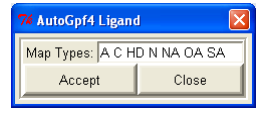
\includegraphics{autogrid4.PNG}
	\end{figure}
	\item Simpan berkas receptor dalam format *.gpf
\end{itemize}

\noindent \textbf{Menghitung atomic affinity maps} \\
Pemetaan yang sudah dilakukan pada receptor dan menghasilkan berkas receptor dalam format *.gpf harus dipetakan untuk setiap berkas ligand. Proses pemetaan ini dilakukan dengan cara menghitung atomic affinity maps pada berkas receptor dengan menggunakan aplikasi autogrid4. Tahapan ini akan menghasilkan berkas pemetaan dalam format *.glg, *.map, *maps.xyz dan *.maps.fld. Untuk mendapatkan hasil tersebut dapat dijalankan \textit{script} berikut pada \textit{desktop} PC yang telah terpasang Autodock Tools : \\
\begin{lstlisting}[caption=\textit{Script} untuk menghitung atomic affinity maps][frame=single]
#!bin/csh
/path/to/autogrid4 -p receptor.gpf -l receptor.glg
\end{lstlisting}
%-----------------------------------------------------------------------------%



\noindent \textbf{Mempersiapkan Docking Parameter Files} \\
Menyiapkan docking parameter files untuk setiap ligand dibantu modul phyton dari Autodock Tools 1.5.2 yang bernama prepare\_dpf4.py. Docking parameter files ini berisi informasi terkait ligand seperti jumlah atom, koordinat
atom dan jumlah torsi aktif yang dimiliki yang sudah dipetakan ke dalam informasi pada receptor. Hasil dari tahapan ini adalah berkas docking parameter files dalam format *.dpf. Jalankan modul prepare\_dpf4.py dengan \textit{script} berikut ini
\begin{lstlisting}[caption=\textit{script} untuk mempersiapkan docking parameter file]
for f in M*.pdbqt;do
name=`basename $f .pdbqt`
echo $name
/path/to/pythonsh /path/to /prepare_dpf.py -l $f -d
/path/to/ligand_dict.py -l `basename $f` -r
receptor.pdbqt \
-p ga_num_evals=1750000 \
-p ga_pop_size=150 \
-p ga_run=20 \
-p rmstol=2.0
End
\end{lstlisting}

\addChapter{Lampiran C}
\chapter*{Lampiran C}

\textbf{Kode yang digunakan dalam menjalankan eksperimen Autodock Vina versi 1.1} \\
\begin{lstlisting}[caption=\textit{Script} yang digunakan pada \textit{desktop} PC host dimana Docker terpasang]
#!/bin/bash

FILES="/percobaan2/*.pdbqt"
COUNTER_FILE=1
COUNTER_CONTAINER=1
NAMA_CONTAINER="vina"
COUNT=1
JUMLAH_FILE=0
LIMIT_FILE=0
RESIDU_FILE=0
JUMLAH_CONTAINER=$1

#menghitung banyaknya file yang dicopy kedalam container
let JUMLAH_FILE=`ls -1 /percobaan2/ | wc -l`
let LIMIT_FILE=$JUMLAH_FILE/$JUMLAH_CONTAINER
let RESIDU_FILE=$JUMLAH_FILE%$JUMLAH_CONTAINER
if [ $RESIDU_FILE -eq 0 ]
then 
let LIMIT_FILE=LIMIT_FILE+0
else
let LIMIT_FILE=LIMIT_FILE+1
fi

#main method
for f in $FILES
do 
if [ $COUNTER_FILE -eq 1 ]
then 
echo "Membuat container" $NAMA_CONTAINER$COUNTER_CONTAINER
docker run -i -t --name $NAMA_CONTAINER$COUNTER_CONTAINER -d agungputrap/riset_docker:latest
CONTAINER_ID=`docker inspect -f '{{.Id}}' $NAMA_CONTAINER$COUNTER_CONTAINER`
echo "ini nomor container = " $CONTAINER_ID
cp /3LP1O.pdbqt /var/lib/docker/aufs/diff/$CONTAINER_ID/3LP1O.pdbqt
cp /conf.txt /var/lib/docker/aufs/diff/$CONTAINER_ID/conf.txt
echo "mengcopy file "$COUNTER_FILE " ke container " $NAMA_CONTAINER$COUNTER_CONTAINER
cp $f /var/lib/docker/aufs/diff/$CONTAINER_ID/`basename $f`
echo "file dicopy " $COUNT
let COUNT=COUNT+1
let COUNTER_FILE=COUNTER_FILE+1
elif [ $COUNT -eq $JUMLAH_FILE ]
then 
echo "harusnya nilai terakhir "$COUNT
echo "mengcopy file terakhir ke container "$NAMA_CONTAINER$COUNTER_CONTAINER
cp $f /var/lib/docker/aufs/diff/$CONTAINER_ID/`basename $f`
cp /running_vina /var/lib/docker/aufs/diff/$CONTAINER_ID/running_vina
docker exec -d $NAMA_CONTAINER$COUNTER_CONTAINER chmod u+x /running_vina
docker exec -d $NAMA_CONTAINER$COUNTER_CONTAINER ./running_vina
elif [ $COUNTER_FILE -lt $LIMIT_FILE ]
then 
echo "mengcopy file "$COUNTER_FILE" ke container "$NAMA_CONTAINER$COUNTER_CONTAINER
cp $f /var/lib/docker/aufs/diff/$CONTAINER_ID/`basename $f`
echo "file dicopy " $COUNT
let COUNT=COUNT+1
let COUNTER_FILE=COUNTER_FILE+1
#case paling terakhir dijalanin
#	elif [ $COUNT -eq $JUMLAH_FILE ]
#	then 
#		echo "harusnya nilai terakhir "$COUNT
#		echo "mengcopy file terakhir ke container"$NAMA_CONTAINER$COUNTER_CONTAINER
#		cp $f /var/lib/docker/aufs/diff/$CONTAINER_ID/`basename $f`
#		cp /running_vina /var/lib/docker/aufs/$CONTAINER_ID/running_vina
#		docker exec -d $NAMA_CONTAINER$COUNTER_CONTAINER chmod u+x /running_vina
#		docker exec -d $NAMA_CONTAINER$COUNTER_CONTAINER ./running_vina
else
#mengcopy file terakhir dalam suatu container dan menjalankan script dalam container
echo "mengcopy file "$COUNTER_FILE" ke container "$NAMA_CONTAINER$COUNTER_CONTAINER
cp $f /var/lib/docker/aufs/diff/$CONTAINER_ID/`basename $f`
echo "file dicopy "$COUNT
let COUNT=COUNT+1
cp /running_vina /var/lib/docker/aufs/diff/$CONTAINER_ID/running_vina
docker exec -d $NAMA_CONTAINER$COUNTER_CONTAINER chmod u+x /running_vina
docker exec -d $NAMA_CONTAINER$COUNTER_CONTAINER ./running_vina
let COUNTER_FILE=1
let COUNTER_CONTAINER=COUNTER_CONTAINER+1
fi
done

\end{lstlisting}

\begin{lstlisting}[caption=\textit{Script} yang digunakan untuk menjalankan aplikasi Autodock Vina dalam container]
#!/bin/bash
FILES="/*.pdbqt"
echo "Waktu mulai " >> logvina.txt
date >> logvina.txt
for f in $FILES
do
./autodockvina/bin/vina --config conf.txt --ligand `basename $f`
done
echo "Waktu selesai " >> logvina.txt
date >> logvina.txt

\end{lstlisting}
\begin{lstlisting}[caption=\textit{Script} yang digunakan untuk mengambil hasil dari menjalankan aplikasi Autodock Vina pada container]
#!/bin/bash
COUNTER_CONTAINER=1
COUNTER=0
NAMA_CONTAINER="vina"
FILES="/var/lib/docker/aufs/diff/"
JUMLAH_FILE=0
let JUMLAH_FILE=`ls -1 /percobaan2/ | wc -l`
while [ $COUNTER -lt $JUMLAH_FILE ];
do
CONTAINER_ID=`docker inspect -f '{{.Id}}' $NAMA_CONTAINER$COUNTER_CONTAINER`
FILEX="$FILES$CONTAINER_ID/*_out.pdbqt"
echo $FILEX
for f in $FILEX
do
docker cp $NAMA_CONTAINER$COUNTER_CONTAINER:`basename $f` /hasilvina/
let COUNTER=COUNTER+1
done
let COUNTER_CONTAINER=COUNTER_CONTAINER+1
done

\end{lstlisting}

\begin{lstlisting}[caption=\textit{Script} yang digunakan untuk mengambil log dari masing - masing container]
#!/bin/bash
COUNTER_CONTAINER=1
COUNTER=0
NAMA_CONTAINER="vina"
FILES="/var/lib/docker/aufs/diff/"
JUMLAH_FILE=$1
while [ $COUNTER -lt $JUMLAH_FILE ];
do
CONTAINER_ID=`docker inspect -f '{{.Id}}' $NAMA_CONTAINER$COUNTER_CONTAINER`
FILEX="$FILES$CONTAINER_ID/logvina*"
echo $FILEX
for f in $FILEX
do
docker cp $NAMA_CONTAINER$COUNTER_CONTAINER:`basename $f` /logvina/$NAMA_CONTAINER$COUNTER_CONTAINER/
let COUNTER=COUNTER+1
done
let COUNTER_CONTAINER=COUNTER_CONTAINER+1
done

\end{lstlisting}

\addChapter{Lampiran D}
\chapter*{Lampiran D}
\textbf{Kode yang digunakan dalam menjalankan eksperimen Autodock versi 4.2} \\

\begin{lstlisting}[caption=\textit{Script} yang digunakan pada \textit{desktop} PC untuk membuat container dan menjalankan container]
#!/bin/bash

FILES="/percobaan2/*.pdbqt"
COUNTER_FILE=1
COUNTER_CONTAINER=1
NAMA_CONTAINER="dock"
COUNT=1
JUMLAH_FILE=0
LIMIT_FILE=0
RESIDU_FILE=0
JUMLAH_CONTAINER=$1

#menghitung banyaknya file yang dicopy kedalam container
let JUMLAH_FILE=`ls -1 /percobaan2/ | wc -l`
let LIMIT_FILE=$JUMLAH_FILE/$JUMLAH_CONTAINER
let RESIDU_FILE=$JUMLAH_FILE%$JUMLAH_CONTAINER
if [ $RESIDU_FILE -eq 0 ]
then 
let LIMIT_FILE=LIMIT_FILE+0
else
let LIMIT_FILE=LIMIT_FILE+1
fi

#main method
for f in $FILES
do 
if [ $COUNTER_FILE -eq 1 ]
then 
echo "Membuat container" $NAMA_CONTAINER$COUNTER_CONTAINER
docker run -i -t --name $NAMA_CONTAINER$COUNTER_CONTAINER -d agungputrap/riset_docker:latest
CONTAINER_ID=`docker inspect -f '{{.Id}}' $NAMA_CONTAINER$COUNTER_CONTAINER`
echo "ini nomor container = " $CONTAINER_ID
cp /3LP1O* /var/lib/docker/aufs/diff/$CONTAINER_ID/
#		memproses ligand menjadi .dpf dan mengcopy ke dalam container beserta ligand
echo "memproses file "$COUNTER_FILE
./home/agungpp/MGLTools-1.5.6/MGLToolsPckgs/AutoDockTools/Utilities24/prepare_dpf4.py -l $f -r /3LP1O.pdbqt 
NAMA=`basename $f .pdbqt`
OUTPUT_PREPARE=$NAMA"_3LP1O.dpf"
cp /$OUTPUT_PREPARE /var/lib/docker/aufs/diff/$CONTAINER_ID/$OUTPUT_PREPARE
echo "mengcopy file "$COUNTER_FILE " ke container " $NAMA_CONTAINER$COUNTER_CONTAINER
cp $f /var/lib/docker/aufs/diff/$CONTAINER_ID/`basename $f`
echo "file dicopy " $COUNT
let COUNT=COUNT+1
let COUNTER_FILE=COUNTER_FILE+1
elif [ $COUNT -eq $JUMLAH_FILE ]
then 
echo "harusnya nilai terakhir "$COUNT
echo "memproses file terakhir "
./home/agungpp/MGLTools-1.5.6/MGLToolsPckgs/AutoDockTools/Utilities24/prepare_dpf4.py -l $f -r /3LP1O.pdbqt
NAMA=`basename $f .pdbqt`
OUTPUT_PREPARE=$NAMA"_3LP1O.dpf"
cp /$OUTPUT_PREPARE /var/lib/docker/aufs/diff/$CONTAINER_ID/$OUTPUT_PREPARE
echo "mengcopy file " $COUNTER_FILE " ke container " $NAMA_CONTAINER$COUNTER_$CONTAINER
cp $f /var/lib/docker/aufs/diff/$CONTAINER_ID/`basename $f`
cp /running_dock /var/lib/docker/aufs/diff/$CONTAINER_ID/running_dock
docker exec -d $NAMA_CONTAINER$COUNTER_CONTAINER chmod u+x /running_dock
docker exec -d $NAMA_CONTAINER$COUNTER_CONTAINER ./running_dock
elif [ $COUNTER_FILE -lt $LIMIT_FILE ]
then 
echo "memproses file " $COUNTER_FILE
./home/agungpp/MGLTools-1.5.6/MGLToolsPckgs/AutoDockTools/Utilities24/prepare_dpf4.py -l $f -r /3LP1O.pdbqt
NAMA=`basename $f .pdbqt`
OUTPUT_PREPARE=$NAMA"_3LP1O.dpf"
cp /$OUTPUT_PREPARE /var/lib/docker/aufs/diff/$CONTAINER_ID/$OUTPUT_PREPARE
echo "mengcopy file "$COUNTER_FILE" ke container "$NAMA_CONTAINER$COUNTER_CONTAINER
cp $f /var/lib/docker/aufs/diff/$CONTAINER_ID/`basename $f`
echo "file dicopy " $COUNT
let COUNT=COUNT+1
let COUNTER_FILE=COUNTER_FILE+1
#case paling terakhir dijalanin
#	elif [ $COUNT -eq $JUMLAH_FILE ]
#	then 
#		echo "harusnya nilai terakhir "$COUNT
#		echo "mengcopy file terakhir ke container"$NAMA_CONTAINER$COUNTER_CONTAINER
#		cp $f /var/lib/docker/aufs/diff/$CONTAINER_ID/`basename $f`
#		cp /running_vina /var/lib/docker/aufs/$CONTAINER_ID/running_vina
#		docker exec -d $NAMA_CONTAINER$COUNTER_CONTAINER chmod u+x /running_vina
#		docker exec -d $NAMA_CONTAINER$COUNTER_CONTAINER ./running_vina
else
#mengcopy file terakhir dalam suatu container dan menjalankan script dalam container
echo "memproses file " $COUNTER_FILE
./home/agungpp/MGLTools-1.5.6/MGLToolsPckgs/AutoDockTools/Utilities24/prepare_dpf4.py -l $f -r /3LP1O.pdbqt
NAMA=`basename $f .pdbqt`
OUTPUT_PREPARE=$NAMA"_3LP1O.dpf"
cp /$OUTPUT_PREPARE /var/lib/docker/aufs/diff/$CONTAINER_ID/$OUTPUT_PREPARE
echo "mengcopy file "$COUNTER_FILE" ke container "$NAMA_CONTAINER$COUNTER_CONTAINER
cp $f /var/lib/docker/aufs/diff/$CONTAINER_ID/`basename $f`
echo "file dicopy "$COUNT
let COUNT=COUNT+1
cp /running_dock /var/lib/docker/aufs/diff/$CONTAINER_ID/running_dock
docker exec -d $NAMA_CONTAINER$COUNTER_CONTAINER chmod u+x /running_dock
docker exec -d $NAMA_CONTAINER$COUNTER_CONTAINER ./running_dock
let COUNTER_FILE=1
let COUNTER_CONTAINER=COUNTER_CONTAINER+1
fi
done

\end{lstlisting}

\begin{lstlisting}[caption=\textit{Script} yang dijalankan pada masing - masing container]
#!/bin/bash
FILES="/*_3LP1O.dpf"
echo "Waktu mulai " >> logdock.txt
date >> logdock.txt
for f in $FILES
do
./autodock/autodock4 -p $f -l `basename $f .dpf`.dlg
done
echo "Waktu selesai " >> logdock.txt
date >> logdock.txt

\end{lstlisting}

\begin{lstlisting}[caption=\textit{Script} yang digunakan untuk mengambil hasil dari menjalankan aplikasi Autodock dari masing - masing container]
#!/bin/bash
COUNTER_CONTAINER=1
COUNTER=0
NAMA_CONTAINER="dock"
FILES="/var/lib/docker/aufs/diff/"
JUMLAH_FILE=0
let JUMLAH_FILE=`ls -1 /percobaan2/ | wc -l`
while [ $COUNTER -lt $JUMLAH_FILE ];
do
CONTAINER_ID=`docker inspect -f '{{.Id}}' $NAMA_CONTAINER$COUNTER_CONTAINER`
FILEX="$FILES$CONTAINER_ID/*.dlg"
echo $FILEX
for f in $FILEX
do
docker cp $NAMA_CONTAINER$COUNTER_CONTAINER:`basename $f` /hasildock/
let COUNTER=COUNTER+1
done
let COUNTER_CONTAINER=COUNTER_CONTAINER+1
done

\end{lstlisting}
\begin{lstlisting}[caption=\textit{Script} yang digunakan untuk mengambil log dari masing - masing container]
#!/bin/bash
COUNTER_CONTAINER=1
COUNTER=0
NAMA_CONTAINER="dock"
FILES="/var/lib/docker/aufs/diff/"
JUMLAH_FILE=$1
while [ $COUNTER -lt $JUMLAH_FILE ];
do
CONTAINER_ID=`docker inspect -f '{{.Id}}' $NAMA_CONTAINER$COUNTER_CONTAINER`
FILEX="$FILES$CONTAINER_ID/logdock*"
echo $FILEX
for f in $FILEX
do
docker cp $NAMA_CONTAINER$COUNTER_CONTAINER:`basename $f` /logdock/$NAMA_CONTAINER$COUNTER_CONTAINER/
let COUNTER=COUNTER+1
done
let COUNTER_CONTAINER=COUNTER_CONTAINER+1
done

\end{lstlisting}